% !TEX root = macfp_2017_gasphase.tex

\subsection{Case 2: Turbulent Pool Fires with Gaseous Fuel} \label{sec:gaseous_pool_fires}

\subsubsection{Experiments}

The gaseous pool fire experiments selected for the first MaCFP workshop correspond to a series of natural gas flame experiments (Case 2a) studied at the National Institute of Standards and Technology (NIST)~\cite{Case2a_EXP} and a series of methane and hydrogen pool fire experiments (Case 2b) studied at Sandia National Laboratories (Sandia)~\cite{Case2b_EXP_CH4,Case2b_EXP_H2}. The original goal of the NIST McCaffrey natural gas flame experiment was to provide data to establish and/or validate engineering correlations for mean temperature and mean vertical flow velocity along the center line of pool fires. The original goal of the Sandia methane and hydrogen pool fire experiment was to provide comprehensive turbulent flow velocity statistics in a configuration that is representative of large-scale pool fires.

The McCaffrey burner is a small-scale (0.3~$\times$~0.3)~m$^2$ square burner; in Ref.~\cite{Case2a_EXP}, the total heat release rate was varied between 14.4 and 57.5~kW. Measurements of temperature and vertical flow velocity were made using thermocouples and bi-directional probes. The Sandia burner is a 1-m-diameter round burner located in a facility that can be approximated as a 6.1~m cube covered by an extraction hood; in Refs.~\cite{Case2b_EXP_CH4,Case2b_EXP_H2}, the total heat release rate was MW-scale (for the purpose of MaCFP, tests no. 14, 24, 17 and 35 were selected corresponding to methane flames with a total heat release rate equal to 1.59, 2.07 and 2.61~MW, and to a hydrogen flame with a total heat release rate equal to 2.12~MW, respectively). The Sandia flames featured strong puffing motions and the formation of thermals. Flow velocities were measured using Particle Image Velocitimetry; starting from the burner surface, measurements were made at high resolution (with a spacing of 2~cm) and over a region approximately 0.9 m~high and 1~m wide. Estimates of errors in mean velocities for tests no. 14, 24, 17 and 35 range between 13\% and 23\%; estimates of errors in {\it rms} velocities range between 13\% and 28\%.

\subsubsection{Simulations}

Four groups submitted computational results for Case 2a: FM Global~\cite{Case2a_SIM_FMG}, UGent~\cite{Case2a_SIM_UGent}, IRSN~\cite{Case2a_SIM_IRSN} and NIST~\cite{Case2a_SIM_NIST}. Four groups submitted computational results for Case 2b: UGent~\cite{Case2b_SIM_UGent}, NIST~\cite{Case2b_SIM_NIST}, SNL~\cite{Case2b_SIM_SNL} and the UCantabria~\cite{Case2b_SIM_UCantabria}. FM Global used a shared development version of FireFOAM (FireFOAM-dev)~\cite{FireFOAM}; UGent used FireFOAM version 2.4.x (Case 2a) and version  2.2.x (Case 2b)~\cite{FireFOAM}; IRSN used ISIS version 4.8.0~\cite{ISIS}; NIST and UCantabria used an official release of FDS (version 6.5.3)~\cite{FDS}; SNL used SIERRA/Fuego version 4.44~\cite{SIERRA/Fuego}.

As discussed in section~\ref{sec:CGD}, the main challenge found in the design of a computational grid for LES simulations of the NIST McCaffrey flame experiment is to provide suitable grid resolution to capture the flow and flame features with length scales comparable to the burner size. All groups responded to this challenge in similar ways: FM Global and UGent adopted a 1.25-cm resolution in the flame zone; IRSN adopted a 1-cm resolution; NIST adopted a 1.43-cm resolution. Furthermore, as discussed in section~\ref{sec:CGD}, the dynamics of the Sandia pool fire experiment are apparently more complex and the main challenge found in the design of a computational grid for LES simulations is to provide suitable grid resolution to capture the intermittent boundary layer flame and thermals that result from the puffing instability. This may require millimeter-scale resolution. Given the high computational cost associated with simulations of meter-size configurations with millimeter-scale resolution, the computational groups responded to this challenge in different ways: UGent and NIST adopted a 1.5-cm resolution in the flame zone; SNL presented results obtained with a 2.5-cm and a 4-cm resolution; UCantabria adopted a 5-cm resolution. Note that while UGent and NIST decided to limit the computational domain to a subset of the experimental facility, SNL and UCantabria chose to include details of the full facility, including the co-flow arrangement and the extraction hood.

Additional differences in the numerical treatment of the NIST McCaffrey and Sandia pool fire experiments include differences in the choice of physical models (see section~\ref{sec:PM} for details on baseline choices). For Case 2a, FM Global used the baseline configuration of FireFOAM except for using a slightly simplified radiation treatment in which emission losses are correctly included in the energy equation (using the global radiative loss fraction concept) but radiation transport is ignored ($i.e.$ the RTE equation is not solved) because comparisons to experimental data do not require the evaluation of a heat flux at a remote surface; the values of the global radiative loss fraction were prescribed using the measured values (varying between 17\% and 27\%). UGent also used the baseline configuration of FireFOAM except for using the dynamic Smagorinsky model~\cite{Moin:1991} for subgrid-scale turbulence; the value of the global radiative loss fraction was prescribed as equal to 20\%; in the solution of the RTE, the discretization of angular space used 48 angles. IRSN used the baseline configuration of ISIS. NIST used the baseline configuration of FDS: the values of the global radiative loss fraction were prescribed using the measured values; in the solution of the RTE, the discretization of angular space used 104 angles.

For Case 2b, UGent used the baseline configuration of FireFOAM except for using the constant-coefficient Smagorinsky model for subgrid-scale turbulence and an emission/absorption treatment of the RTE for radiation combined with a grey model (for methane flames, the global radiative loss fraction was predicted to be equal to 24.8\%); in the solution of the RTE, the discretization of angular space used 48 angles (additional information can be found in Ref.~\cite{Maragkos:2017}). NIST and UCantabria used the baseline configuration of FDS (except that UCantabria used the Vreman model~\cite{FDS_Math_Guide} for subgrid-scale turbulence): the value of the global radiative loss fraction was prescribed as equal to 20\% (for methane flames) or 10\% (for hydrogen flames); in the solution of the RTE, the discretization of angular space used 104 angles. SNL used the baseline configuration of SIERRA/Fuego (but without radiation).

\begin{figure}
\centering
(a)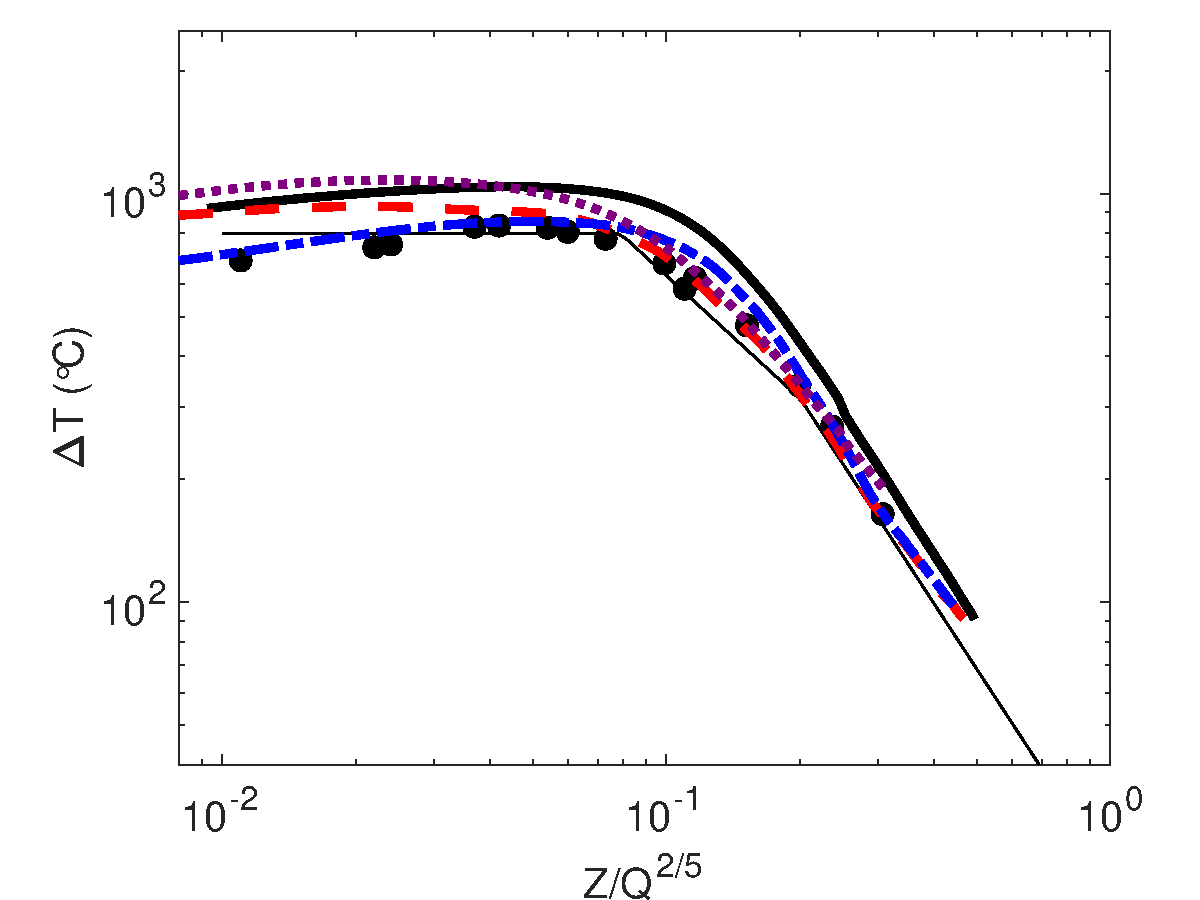
\includegraphics[height=2.2in]{Figures/Case2-Fig1a.pdf}
(b)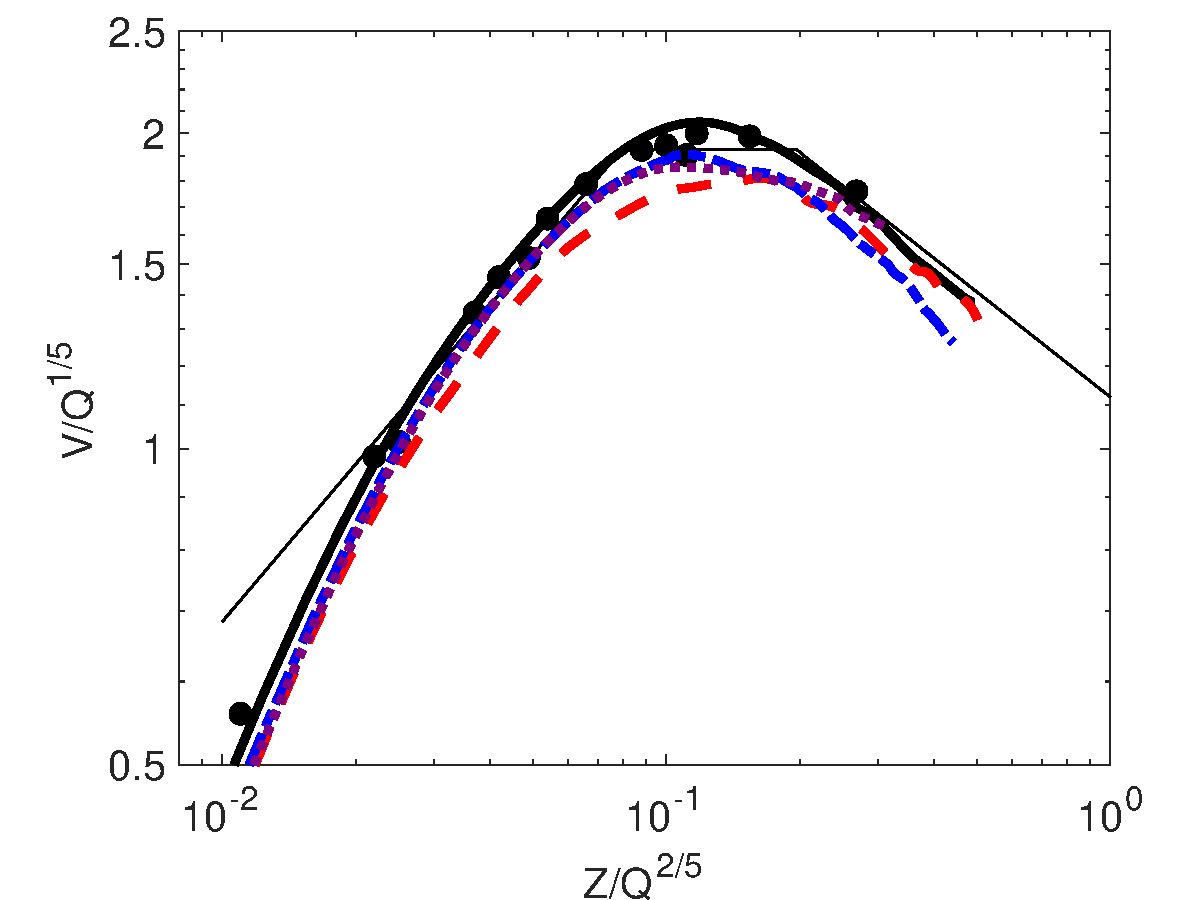
\includegraphics[height=2.2in]{Figures/Case2-Fig1b.pdf}
\caption{Case 2a. Vertical variations along the pool centerline (log-log plot): (a) mean excess temperature; (b) mean vertical velocity. Following standard scaling laws, vertical elevation is scaled by ${Q}^{2/5}$ while velocity is scaled by ${Q}^{1/5}$, with $Q$ the total heat release rate. Comparison between experimental data (black circles), engineering correlations (thin black solid line, see Ref.~\cite{Case2a_EXP}) and numerical results from FM Global (black solid line), IRSN (red dashed line), NIST (blue dash-dotted line), UGent (magenta dotted line). Case of a 33-kW flame.}
\label{fig:Case2-Fig1}
\end{figure}

\subsubsection{Summary}

For Case 2a, all simulations seem to correctly reproduce the gross features of the flame structure observed in the NIST McCaffrey flame experiment. Figure~\ref{fig:Case2-Fig1} presents a representative sample of comparisons between measured and simulated temperatures and vertical flow velocity. Note that in the NIST McCaffrey experiment, thermocouple measurements were not corrected for radiation losses and therefore should be interpreted with caution. NIST is the only computational group that used a thermocouple model to provide a sound basis for comparisons to the raw thermocouple measurements (the model is integrated inside the LES solver and uses the LES solution to simulate deviations of thermocouple temperatures from gas temperatures~\cite{FDS_Math_Guide}); other groups reported gas temperatures that require a correction before making a comparison to the raw thermocouple measurements.

It is worth emphasizing that while the experimental database describing the NIST McCaffrey natural gas flame experiment is a valuable starting point for model validation, there are, however, some obvious limitations in the database that are worth pointing out for future studies: (1) the database is limited to small-scale, weakly-to-moderately turbulent flames; and (2) the database is limited to temporal means and does not contain information on fluctuation magnitudes.

We now proceed to a discussion of Case 2b. All simulations seem to correctly reproduce the gross features of the flame structure observed in the Sandia pool fire experiment. Figures~\ref{fig:Case2-Fig2}-\ref{fig:Case2-Fig3} present a representative sample of comparisons between measured and simulated mean vertical and radial velocities. Mean radial velocities are particularly important because they provide a measure of the air entrainment process that determines the vertical mass flow rate in the flame and plume regions (and thereby controls smoke production in fires): for instance, Figure~\ref{fig:Case2-Fig3} shows that at the edge of the pool fire ($i.e.$ at 0.5-m distance from the center of the burner), the radial velocity is over-estimated by a factor close to two in the SNL and UCantabria simulations (at $z = 0.3$~m). Additional comparisons can be found in~\cite{MaCFP_wks_presentations}. Overall, the UGent and NIST simulations show good agreement with experimental data and provide a satisfactory description of the flame structure. The accuracy of the UCantabria simulation is limited by insufficient grid resolution. 

It is worth emphasizing that the experimental database describing the Sandia methane and hydrogen pool fire experiment is quite unique because it contains data on first and second-order statistical moments of vertical/radial velocities measured with high spatial resolution~\cite{Case2b_EXP_CH4,Case2b_EXP_H2}. There are also some limitations in the database that are worth pointing out for future studies: (1) the Sandia database is limited to the flame near-field, $i.e.$ to low elevations ($z \leq 0.9$~m, $i.e.$ $z < D$), and there is a need to provide data over the full flame region ($0 \leq z \leq L_f$); (2) the Sandia database focuses on the flow structure in the flame region but does not contain information on the temperature and radiation fields.

Finally, it is also worth noting that while research-level simulations may accept the computational cost associated with millimeter- or centimeter-scale resolution, engineering-level simulations will not accept that cost and will use coarser grids ($i.e.$ grids that resolve length-scales on the order of the pool diameter $D$, but not the smaller length scales associated with a boundary layer flame or the presence of thermals). These coarser-grid simulations require accurate subgrid-scale models: the evaluation of current SGS models in simulations with representative engineering-level grids was not part of the scope of the first MaCFP workshop and will be addressed in future editions.


\begin{figure}
\centering
(a)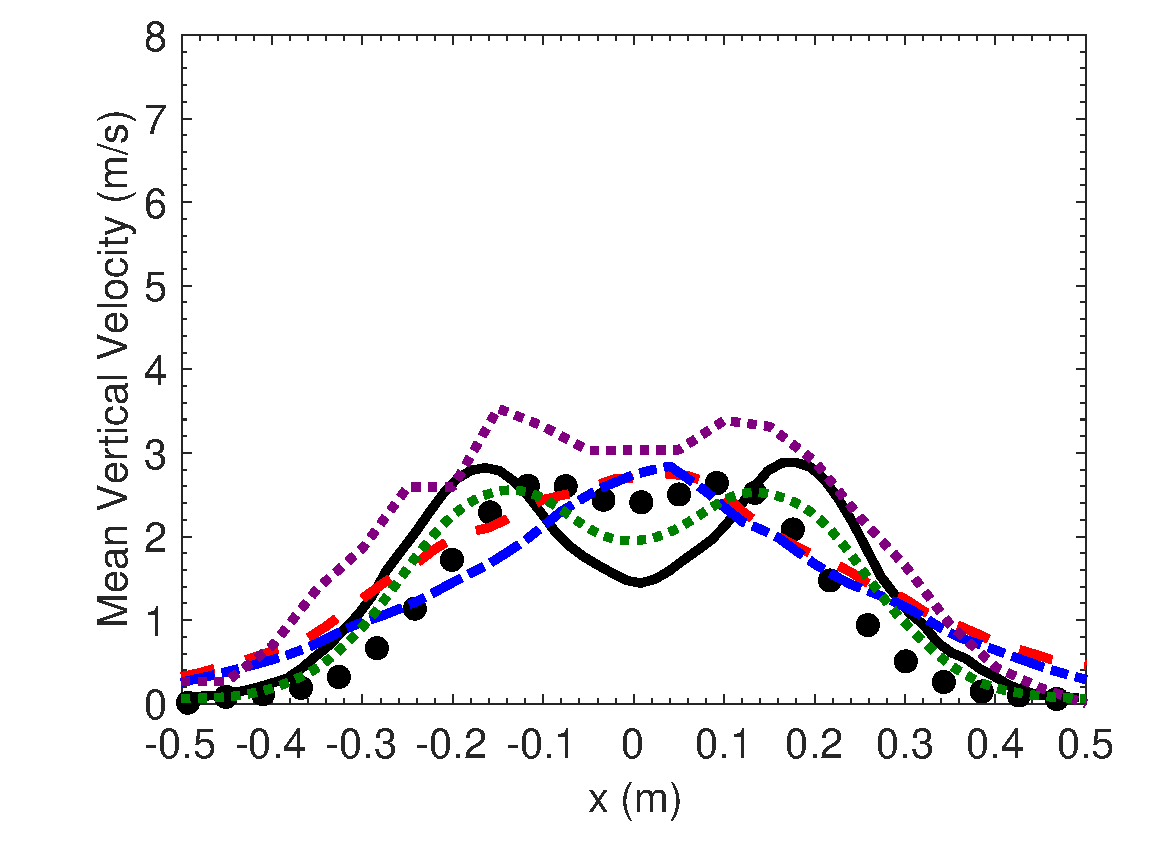
\includegraphics[height=2.2in]{Figures/Case2-Fig2a.pdf}
(b)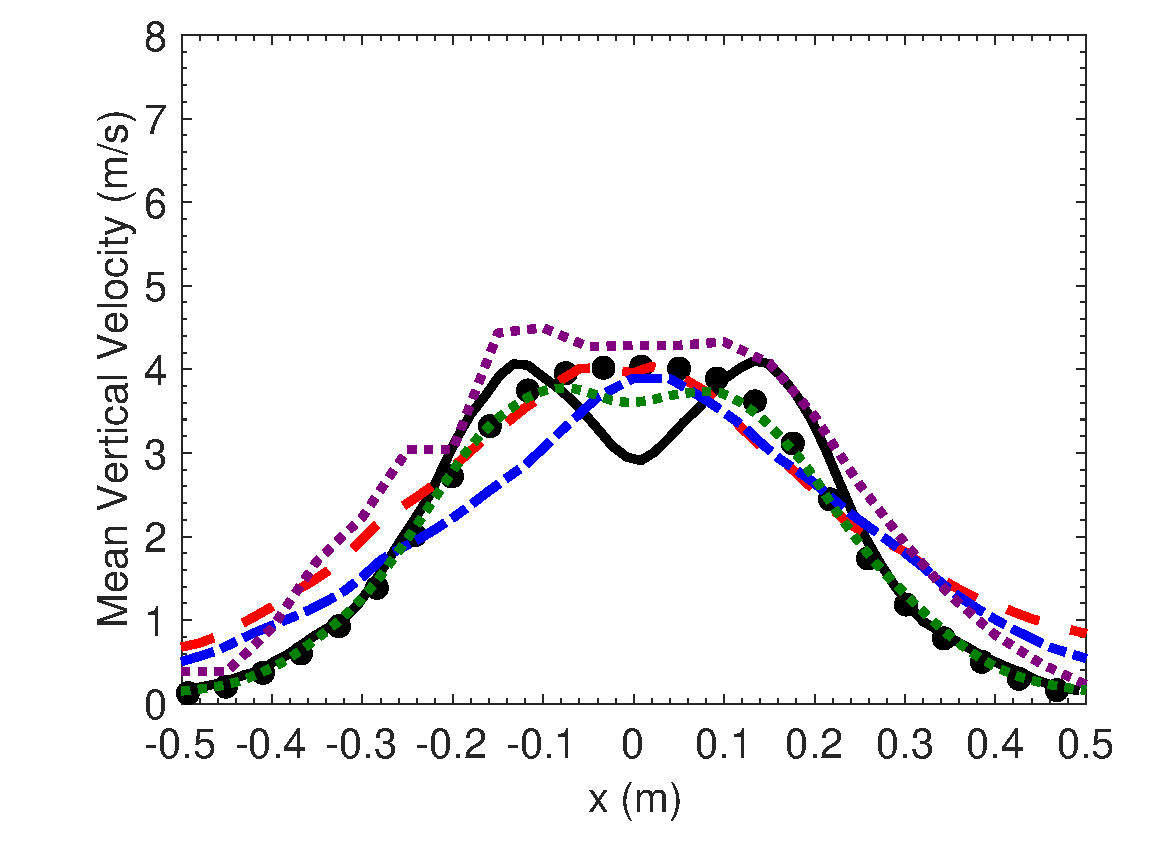
\includegraphics[height=2.2in]{Figures/Case2-Fig2b.pdf}
(c)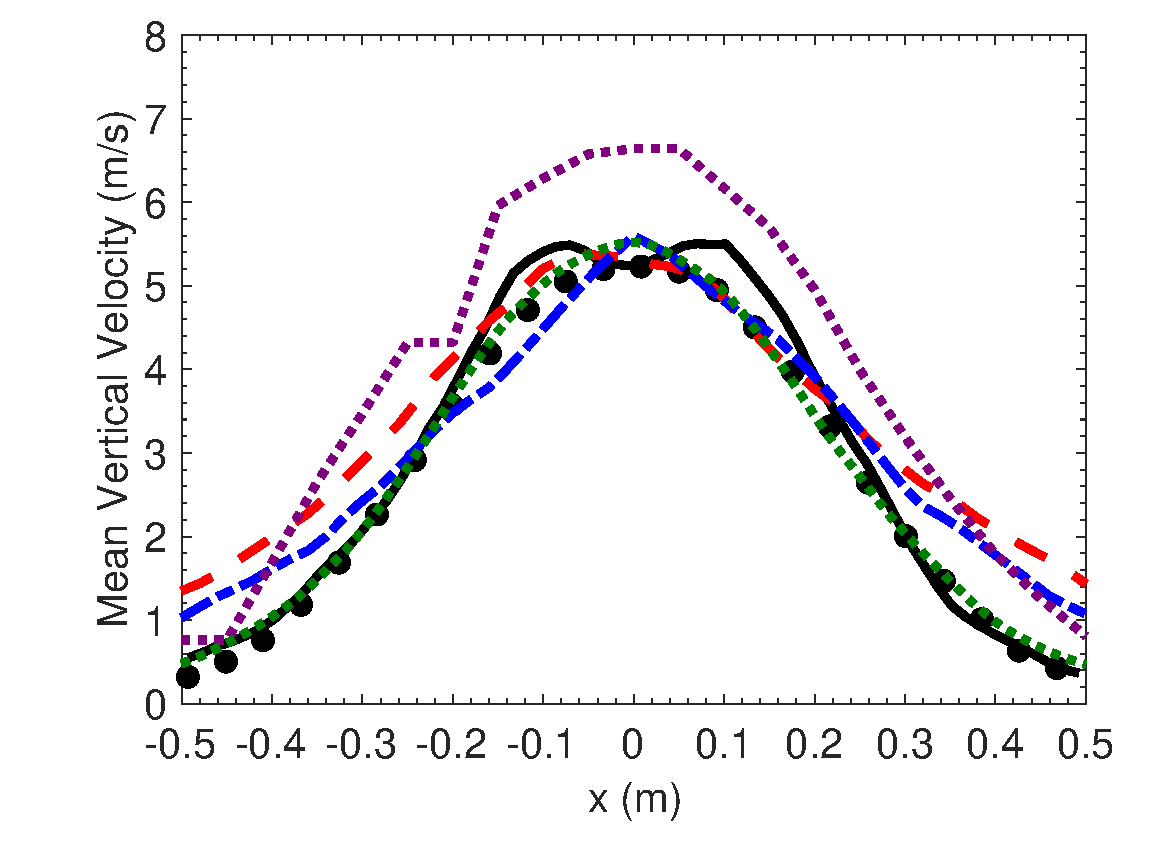
\includegraphics[height=2.2in]{Figures/Case2-Fig2c.pdf}
(d)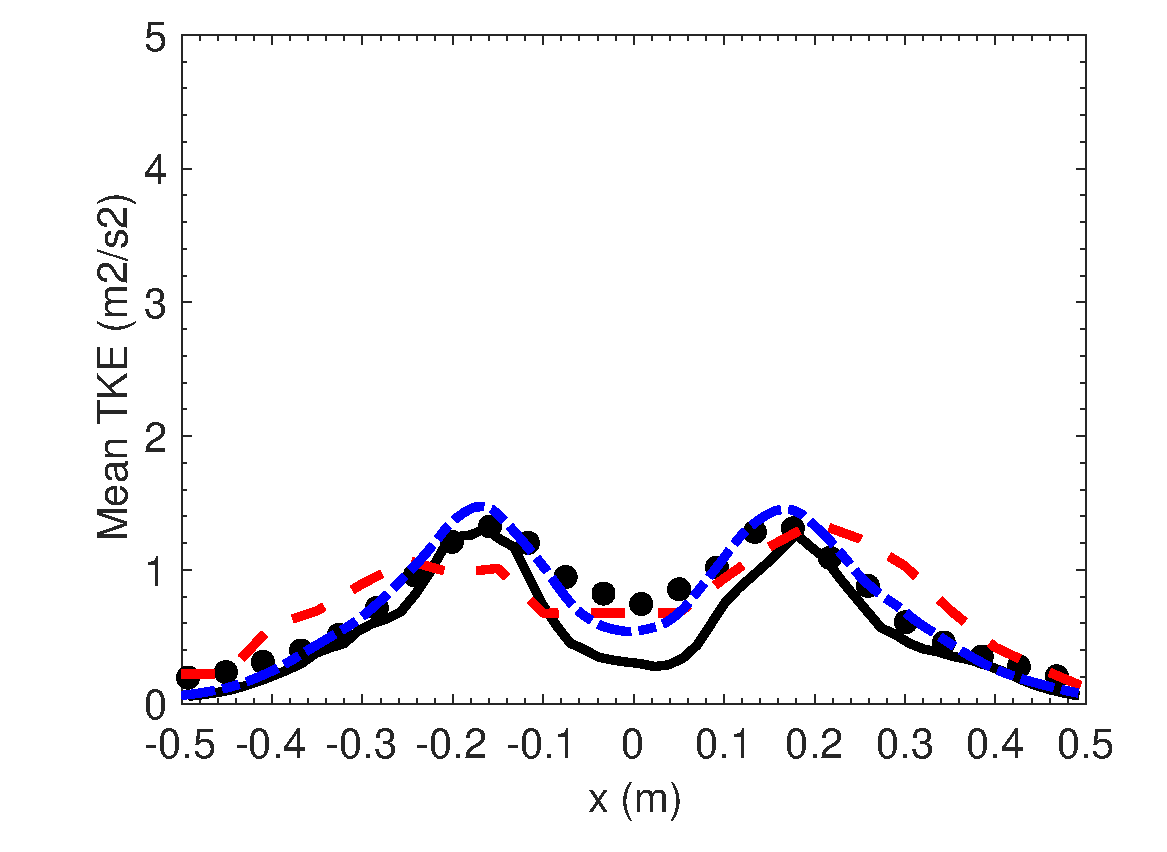
\includegraphics[height=2.2in]{Figures/Case2-Fig2d.pdf}
\caption{Case 2b. Radial variations of mean vertical velocity at elevation: (a) $z = 0.3~m$; (b) $z = 0.5~m$; (c) $z = 0.9~m$; and radial variations of mean (resolved) turbulent kinetic energy at $z = 0.5~m$. Comparison between experimental data (black circles) and numerical results from NIST (black solid line),  SNL (red dashed and blue dash-dotted  lines); UCantabria (magenta dotted line); UGent (green dotted line). Case of a 2.07-MW methane flame (test 24).}

\label{fig:Case2-Fig2}
\end{figure}
\begin{figure}
\centering
(a)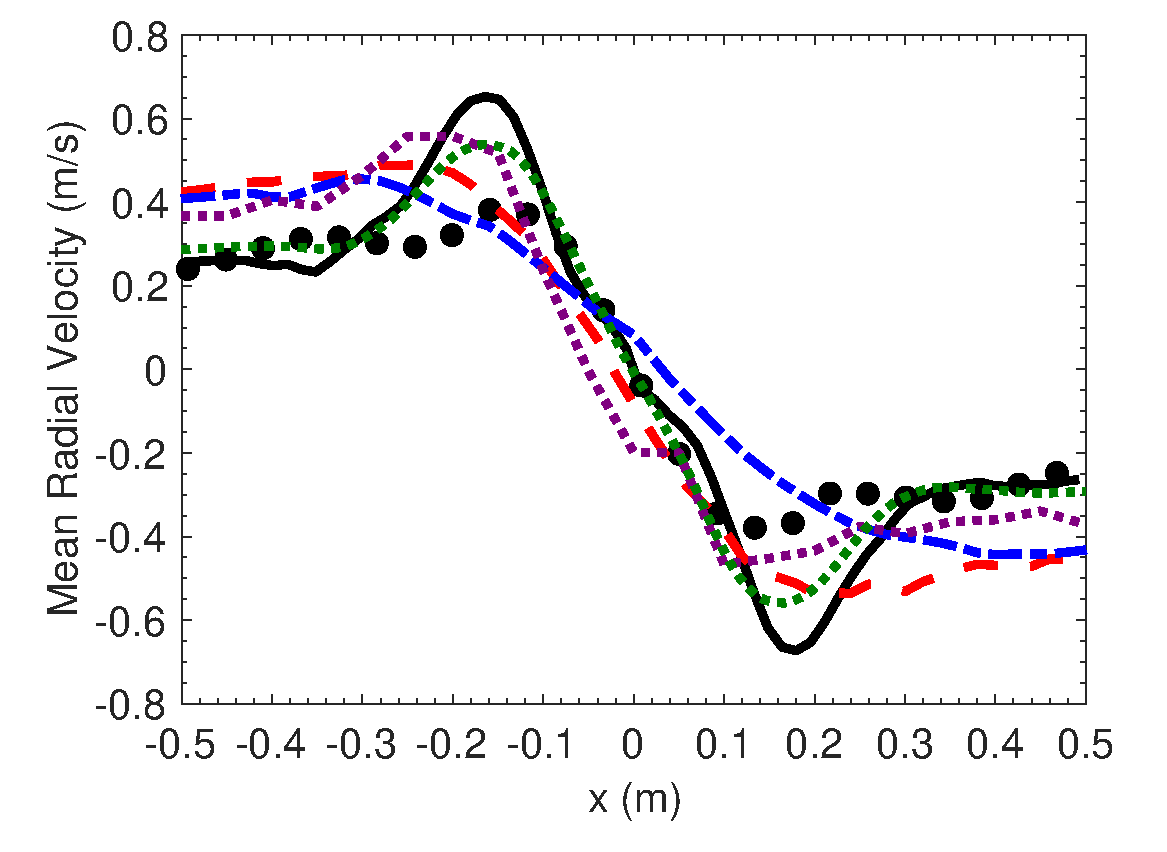
\includegraphics[height=2.2in]{Figures/Case2-Fig3a.pdf}
(b)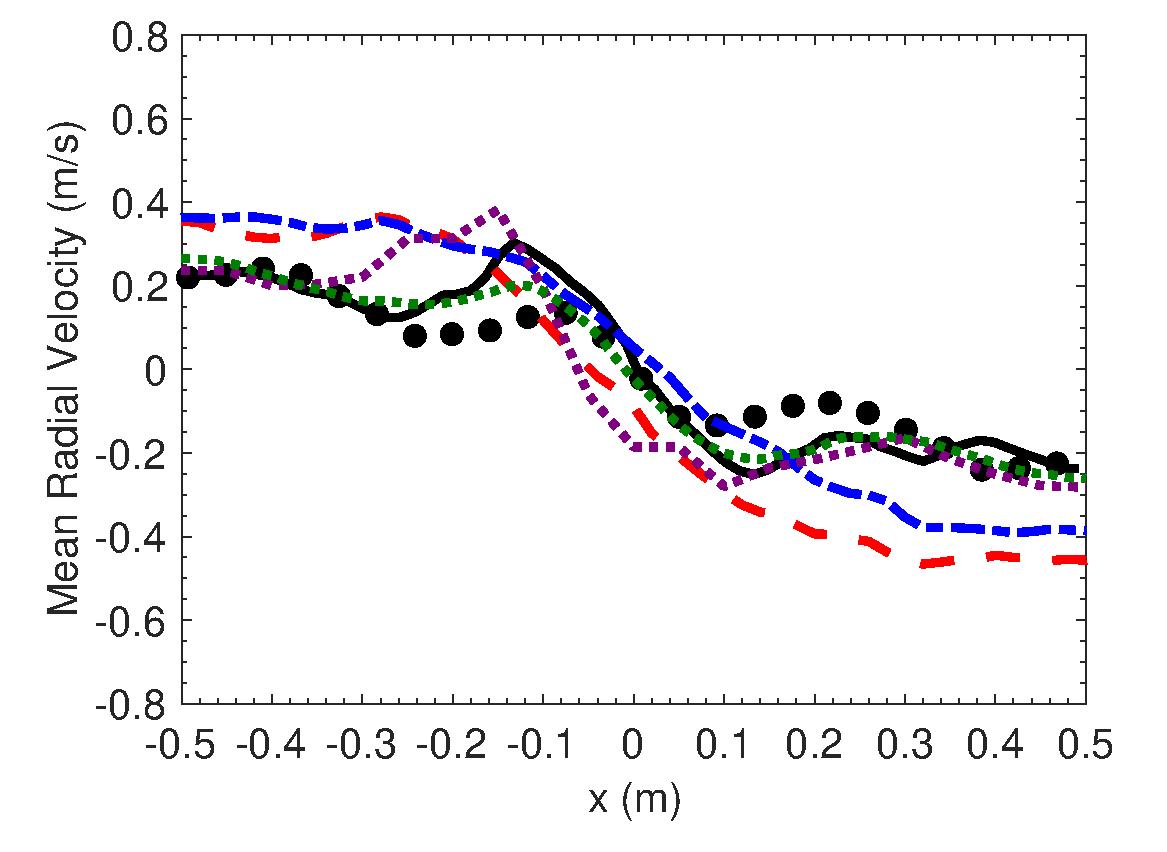
\includegraphics[height=2.2in]{Figures/Case2-Fig3b.pdf}
\caption{Case 2b. Radial variations of mean radial velocity at elevation: (a) $z = 0.3~m$; (b) $z = 0.5~m$. See caption of Fig.~\ref{fig:Case2-Fig2}.}
\label{fig:Case2-Fig3}
\end{figure}


